% Supplementary material for main.tex. It collects what the paper leaves out:
% how the design developed, the parts and costs, the actuation sequence, the
% timing measurements, and the detailed test results. Every number is taken
% from our course reports; where the final code differs, the text says so.
\documentclass[conference]{IEEEtran}
\IEEEoverridecommandlockouts

\usepackage{cite}
\usepackage{booktabs}
\usepackage{graphicx}
\usepackage{listings}
\usepackage{hyperref}

\lstset{basicstyle=\ttfamily\footnotesize, columns=fullflexible, keepspaces=true, frame=tb, xleftmargin=0.5em}

\begin{document}

\title{Vision-Based Connect-4 Robot: Supplementary Material}

\author{%
\IEEEauthorblockN{Andrew Abdelmalak, Daniel Boules, David Girgis,\\Kirolous Kirolous, Samir Yacoub, and Youssef Salama}
\IEEEauthorblockA{\textit{Dept. of Mechatronics Engineering, German University in Cairo}\\
Cairo, Egypt}
}

\maketitle

\begin{abstract}
This document accompanies our paper, \emph{Vision-Based Connect-4 Robot: Closed-Loop Game-State Extraction and Verified Token Placement}. It collects the material the paper leaves out: how the design developed from a literature review to the final build, the parts and costs of the earlier and final designs, the dispenser's actuation sequence, per-operation timing on the Raspberry Pi, and detailed drop, timing, and scenario results. All numbers come from the reports we wrote during the project. Where the final code uses different values, the text gives the code's values.
\end{abstract}

\section{How the Design Developed}

\subsection{Literature Review}
We began by surveying three research threads that a vision-guided Connect-4 robot depends on: board detection and game-state extraction~\cite{Wolflein2021,Masouris2023}, token colour segmentation under changing light~\cite{Akis2024,Ayub2020}, and manipulators for board games~\cite{Matuszek2011}. The paper's related-work section discusses these works. The review fixed one design constraint early. Connect-4 tokens fall under gravity once released above a column, so the robot needs no grasping motion, only repeatable placement along one horizontal axis with an error below half the column pitch, about 20~mm on a standard board.

\subsection{Image Pipeline and First Hardware}
Next, we built and tested each image operation on a sample board photo: rotation and perspective warp, each with nearest-neighbour and bilinear interpolation; a brightness shift and contrast scaling, each checked with histograms; and Gaussian smoothing at $3\times3$, $5\times5$, and $7\times7$ against a box filter. Bilinear interpolation removed the jagged cell boundaries that nearest-neighbour sampling produced. The repository's image-pipeline notebook reproduces these comparisons.

Two image features were defined to drive the actuator: the mean board brightness and the board's rotation angle. On our test image the mean brightness was 91.19, which mapped to a motor speed of about 35\% PWM duty. An Arduino prototype turned a servo from these two values; it is in the repository as \texttt{arduino/servo\_prototype}.

The first mechanism, modelled in SolidWorks, held a stack of tokens over a slide. A DC motor with an end effector pushed out the bottom token, and a servo-driven gate covered the columns that the token should pass, so that it slid into the target column. The planned electronics drove NEMA~17 stepper motors through L298N drivers. Table~\ref{tab:cost} lists the cost of this design.

\subsection{Closed-Loop Integration}
We then connected the stages into one loop: the Raspberry Pi reads the board, plans a move, and sends the column to the Arduino over USB serial, and a Flask dashboard shows the live camera streams. This version still used the stepper motors and the servo gate. Fig.~\ref{fig:circuit} shows the circuit we simulated in Proteus for it.

\begin{figure}[t]
\centering
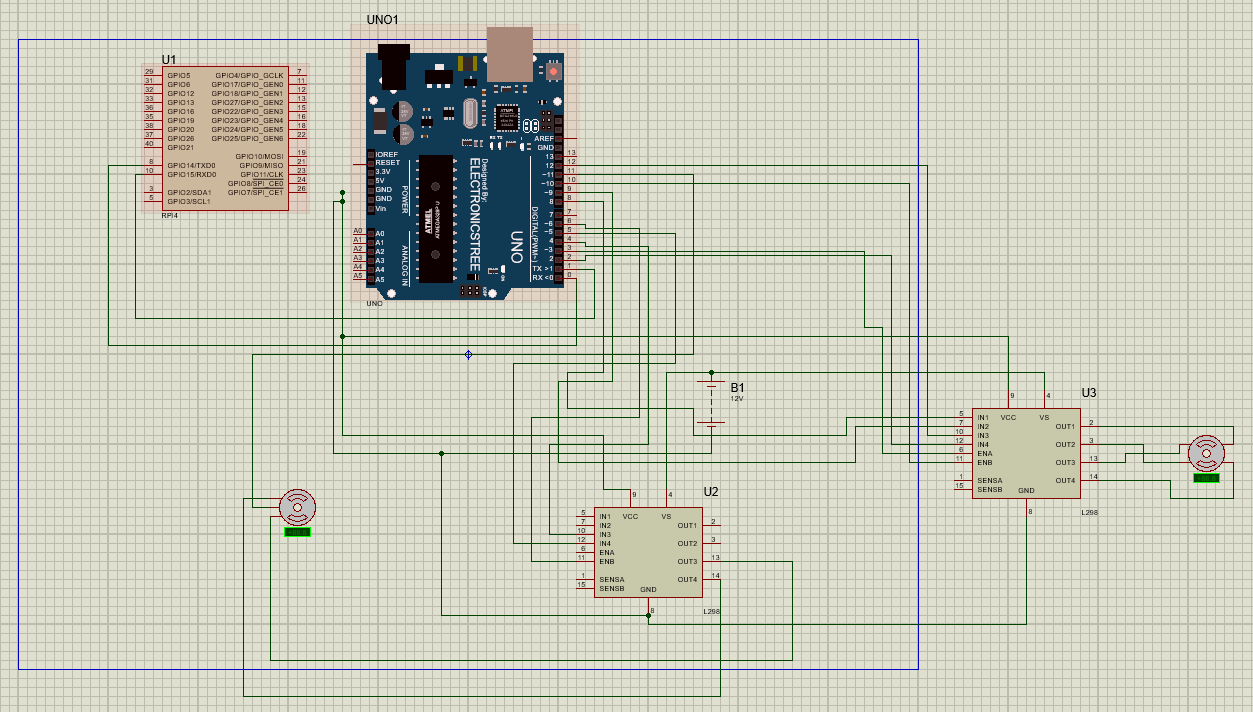
\includegraphics[width=\columnwidth]{figures/proteus_circuit.png}
\caption{Circuit simulated in Proteus for the closed-loop stage: the Arduino Uno, two L298N H-bridge modules for the motors, a 12~V supply, and the servo for the column gate.}
\label{fig:circuit}
\end{figure}

\subsection{Final Build}
Closed-loop testing showed that a simpler split was more repeatable: a time-based carriage driven by a TT geared DC motor, and an encoder-coupled DC motor that releases exactly one token per turn of its disk. The carriage is a rod inside an open rail along the top of the board. At rest it waits out of the board, past the storage end, so every hole is open for the player. Column~1 sits under the chute and needs no move; for column~$N$ the rod slides out over columns~1 to $N-1$, so the released token rolls along it by gravity and drops through column~$N$, the first open hole. The rod then returns out of the board. The servo and the steppers were removed. The final build cost 6,100~EGP (Table~\ref{tab:cost}).

\begin{table}[t]
\caption{Parts and cost of the earlier and final designs (EGP)}
\label{tab:cost}
\centering
\small
\begin{tabular}{lcr}
\toprule
\textbf{Component} & \textbf{Qty} & \textbf{Total} \\
\midrule
\multicolumn{3}{l}{\emph{Earlier design: steppers and a servo gate}} \\
Raspberry Pi 4 (4~GB) & 1 & 5,950 \\
Arduino Uno & 1 & 450 \\
Pi Camera V2 & 1 & 2,150 \\
NEMA 17 stepper motor & 2 & 880 \\
L298N driver & 2 & 170 \\
SG90 micro servo & 1 & 85 \\
12~V 5~A power supply & 1 & 300 \\
Wires and breadboard & 1 & 150 \\
\textbf{Total} & & \textbf{10,135} \\
\midrule
\multicolumn{3}{l}{\emph{Final build: carriage and magazine}} \\
Raspberry Pi 4 (4~GB) & 1 & 4,250 \\
Arduino Uno & 1 & 450 \\
Pi Camera 5MP Rev 1.3 & 1 & 275 \\
TT geared DC motor (carriage) & 1 & 50 \\
Encoder DC motor (magazine) & 1 & 420 \\
L298N H-bridge driver & 1 & 75 \\
12~V 1.2~A power supply & 1 & 50 \\
Wires, breadboard, structural parts & -- & 530 \\
\textbf{Total} & & \textbf{6,100} \\
\bottomrule
\end{tabular}
\end{table}

\section{Actuation Sequence}
The Pi sends one ASCII digit, `1' to `7', at 9600~baud. Fig.~\ref{fig:sequence} shows how the sketch that ran in the demonstrations handles each move. The repository's \texttt{arduino/dispenser/dispenser.ino} is rebuilt from this sequence, because the original file was not kept.

\begin{figure}[t]
\begin{lstlisting}
on serial input c in '1'..'7' and not busy:
  column <- c - '0'; busy <- true
  emit "BUSY column"
  // 1. move the carriage to the column
  drive carriage out for duration[column] ms
  hard-brake carriage; wait 2000 ms
  // 2. release exactly one token
  pulses <- 0; drive magazine motor at fastSpeed
  while pulses < 430:
    if pulses >= 430 - 40: magazine at slowSpeed
  hard-brake magazine; emit "MAG_PULSES pulses"
  wait 500 ms
  // 3. return the carriage home
  drive carriage back for the same time; hard-brake
  busy <- false; emit "DONE column"
\end{lstlisting}
\caption{The dispenser's per-move sequence, as pseudocode of the sketch that ran in the demonstrations.}
\label{fig:sequence}
\end{figure}

The magazine motor turns its disk about 1.075 times per release (430 encoder pulses at 400 counts per turn), which pushes the bottom token out of the storage tube. Hard braking drives both H-bridge inputs high for 100~ms before disabling the channel; it removed coasting and was a key source of repeatable positioning. Table~\ref{tab:carriage} lists the calibrated carriage times.

\begin{table}[t]
\caption{Calibrated carriage drive time per column}
\label{tab:carriage}
\centering
\small
\begin{tabular}{ccc}
\toprule
\textbf{Column} & \textbf{Drive (ms)} & \textbf{Round trip (ms)} \\
\midrule
1 & 0 & 0 \\
2 & 330 & 660 \\
3 & 600 & 1,200 \\
4 & 900 & 1,800 \\
5 & 1,200 & 2,400 \\
6 & 1,500 & 3,000 \\
7 & 1,800 & 3,600 \\
\bottomrule
\end{tabular}
\end{table}

\section{Timing on the Raspberry Pi}
Each pipeline operation was timed over 100 iterations on the Pi and on a laptop for reference (Table~\ref{tab:bench}). Both produce bit-for-bit identical images; the Pi is limited in throughput only. The brightness and contrast settings in the table are the ones used for this benchmark; the robot's code applies a brightness shift of +20 and a contrast gain of 1.3. Minimax at depth~5 typically took 0.2 to 1.4~s on the Pi in the early game, where the branching factor is highest, and less than 0.5~s in later positions.

\begin{table}[t]
\caption{Per-operation execution time, mean of 100 iterations (ms)}
\label{tab:bench}
\centering
\small
\begin{tabular}{lrr}
\toprule
\textbf{Operation} & \textbf{Pi 4} & \textbf{Laptop} \\
\midrule
Rotation (bilinear) & 8.468 & 3.273 \\
Perspective warp & 3.596 & 1.768 \\
Brightness +60 & 0.734 & 0.888 \\
Contrast $\alpha = 1.8$ & 1.111 & 0.201 \\
Gaussian blur $5\times5$ & 0.757 & 0.097 \\
\bottomrule
\end{tabular}
\end{table}

\section{Detailed Results}

\subsection{Token Drops by Column}
Each column received 20 drop trials; a drop succeeded when the token landed in the commanded column (Table~\ref{tab:drops}). The misses on the far columns, toward column~7, come from drift in the time-based carriage positioning.

\begin{table}[t]
\caption{Drop success by column}
\label{tab:drops}
\centering
\small
\begin{tabular}{ccc}
\toprule
\textbf{Column} & \textbf{Trials} & \textbf{Success} \\
\midrule
1 & 20 & 100\% \\
2 & 20 & 100\% \\
3 & 20 & 100\% \\
4 & 20 & 95\% \\
5 & 20 & 95\% \\
6 & 20 & 90\% \\
7 & 20 & 85\% \\
\midrule
All & 140 & 95\% \\
\bottomrule
\end{tabular}
\end{table}

\subsection{End-to-End Time}
End-to-end time runs from an accepted board to the moment the camera verifies the new token in the commanded column. It ranged from 3.0~s at best to 15.0~s at worst, with an average of 7.5~s. The average case breaks down roughly as: 0.05~s vision, 0.01~s validation, 0.95~s minimax, 0.9~s carriage stroke out (middle columns), 2.0~s carriage pause, 0.7~s magazine release, 0.5~s settle, 0.9~s carriage stroke back, and 1.5~s verification. Moves to the home column skip both carriage strokes and finish in about 3~s; the slowest moves combine a far-column stroke with a verification retry after a borderline detection.

\subsection{Closed-Loop Scenarios}
\begin{itemize}
\item \emph{Mid-game states.} Each of the 12 predefined simulator states was set up on the board, captured by the camera, and compared with the expected board. The validator accepted every legal change and rejected every injected illegal one, such as a chip floating two rows above the lowest empty row.
\item \emph{Glare.} A handheld light was swept across the board mid-game. The corner smoothing kept the warp stable; one or two frames gave spurious cell readings, and the validator rejected them without touching the trusted board. Clean readings returned within 1 to 2 frames after the light moved away.
\item \emph{Outer-column stress.} Twenty column-7 commands were sent in a row from a fresh board. Seventeen tokens landed in column 7 and three slipped into column 6; the camera check caught all three, and the robot stopped in its error state until reset.
\end{itemize}

\subsection{Demonstration Video}
Our final demonstration was recorded on video: three moves by a person and three by the robot, with the dashboard on a laptop beside the board. The project page shows a 20-second excerpt.

\section*{Acknowledgment}
We thank Assoc.~Prof.~Dr.~Eng.~Omar M. Shehata, Eng.~Dalia M. Mahfouz, PhD, Eng.~Abdelrahman Hatem, MSc., and Eng.~Mohammed Ashraf for their guidance.

\bibliographystyle{IEEEtran}
\bibliography{references}

\end{document}
